\documentclass[10pt]{beamer}

\usetheme[progressbar=frametitle]{metropolis}
\usepackage{appendixnumberbeamer}

\usepackage{booktabs}
\usepackage[scale=2]{ccicons}

\usepackage{amssymb}

\usepackage{pgfplots}
\usepgfplotslibrary{dateplot}

\usepackage{xspace}
\newcommand{\themename}{\textbf{\textsc{metropolis}}\xspace}

\title{Deep Active Learning for Interactive 3D Segmentation Of Medical Images}
% \date{\today}
\date{\today}
\author{Vincent Groff}
% \titlegraphic{\hfill
\includegraphics[height=1.5cm]{logo.pdf}}

\begin{document}

\maketitle

\begin{frame}{Table of contents}
  \setbeamertemplate{section in toc}[sections numbered]
  \tableofcontents[hideallsubsections]
\end{frame}


%%%%%%%%%%%%%%%%%%%%%%%%%%%%%%%%%%%%%%%%%%%%%%%%%%%%%%%%%%%%%%%%%%%%%%%%%%%%%%%%%%%%
%%%%%%%%%%%%%%%%%%%%%%%%%%%%%%%%%%%%%%%%%%%%%%%%%%%%%%%%%%%%%%%%%%%%%%%%%%%%%%%%%%%%
%%%%%%%%%%%%%%%%%%%%%%%%%%%%%%% Segmentation %%%%%%%%%%%%%%%%%%%%%%%%%%%%%%%%%%%%%%%
%%%%%%%%%%%%%%%%%%%%%%%%%%%%%%%%%%%%%%%%%%%%%%%%%%%%%%%%%%%%%%%%%%%%%%%%%%%%%%%%%%%%
%%%%%%%%%%%%%%%%%%%%%%%%%%%%%%%%%%%%%%%%%%%%%%%%%%%%%%%%%%%%%%%%%%%%%%%%%%%%%%%%%%%%

\section{3D Image Segmentation}

\begin{frame}[fragile]{Medical Image Segmentation}

    \begin{block}{3D Medical Image Segmentation}
    \end{block}
    
    \begin{figure}[h!]
    \centering
    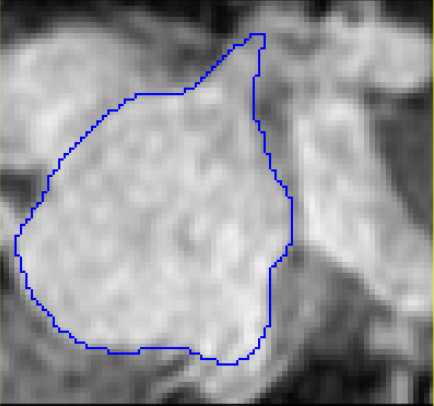
\includegraphics[scale=0.20]{pictures/seg}
    \caption{Segmentation of the left atrium}
    \label{fig:heartSegTruth}
    \end{figure}
        
    \textbf{Main Problem:} Laborious, particularly in 3D
    \pause
    
    \textbf{How can we automate this?}
\end{frame}


\begin{frame}[fragile]{Conditional Random Fields}

    \textbf{Aim:} Separate the set of \textit{background} pixels (\textbf{B}) from the set of \textit{object} pixels (\textbf{O})
  
    \textbf{Define a cost function to be minimized over image $\mathbf{X}$} \cite{graphCuts}
    \pause
    \begin{equation}
      E(\mathbf{X}) = \sum_{i} R_{i} + \lambda \sum_{i} \sum_{j} B_{ij}
      \label{eq:costFunc}
    \end{equation}

    \begin{itemize}
    \item $R_{i}$ - \textbf{Regional Penalty Term} - penalty for assigning pixel $i$ to either the background (\textbf{B}) or object (\textbf{O})
    \item $B_{ij}$ - \textbf{Boundary Penalty Term} - penalty depending on properties of pixels $i$ and $j$
    \item $\lambda > 0$ - a relative weighting
    \end{itemize}
\end{frame}

\begin{frame}[fragile]{Conditional Random Fields}

  
  $R_{i}$ - \textbf{Regional Penalty Term}

  Map (0,1) probabilities to ($\infty$, 0) penalties with negative log
  \begin{equation} R_{i} = \begin{cases} 
      -\log P(i \in O) & i \in \mathbf{O} \\
      -\log P(i \in B) & i \in \mathbf{B} \\
   \end{cases}
  \end{equation}

  \pause
  
  $B_{ij}$ - \textbf{Boundary Penalty Term}

  Want to encourage boundaries at discontinuities in intensity
  
  \textbf{Penalize boundaries that are placed between similar pixels}

  \begin{equation} B_{ij} = \begin{cases}
      0 & y_{i} = y_{j} \\
      \frac{1}{r_{ij}} e^{\frac{-(X_{i}-X_{j})^2}{2\sigma^2}} & y_{i} \neq y_{j} \\
    \end{cases}
    \label{eq:boundTerm}
  \end{equation}

  \begin{itemize}
  \item $X_{i}$ - grayscale value at pixel $i$
  \item $y_{i}$ - binary label for pixel $i$ (0 means $i \in \mathbf{B}$)
  \item $r_{ij}$ - euclidean distance between pixels $i$ and $j$
  \end{itemize}
    
\end{frame}


\begin{frame}[fragile]{Graph Cuts}

  \textbf{How do we get $P(i \in B)$ and $P(i \in O)$?}
  
  \textbf{User interaction}
  
  \begin{itemize}
  \item User gives seed points
  \item Probability distribution produced from seed points
  \item Probabilities of other pixels inferred from distribution
  \end{itemize}
  
  \textbf{Works well, but...}

  \pause
  \textbf{Requires object and background pixels to have distinct intensity values}
  
\end{frame}


\begin{frame}[fragile]{Graph Cuts}

  \textbf{Requires object and background pixels to have distinct intensity values}
   
  \begin{figure}[h!]
    \centering
    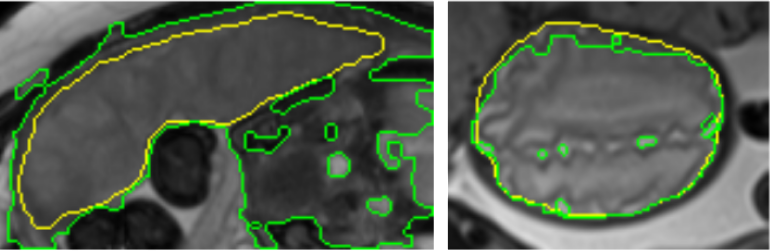
\includegraphics[scale=0.25]{pictures/grabcuts1}
  \end{figure}

     
  \begin{figure}[h!]
    \centering
    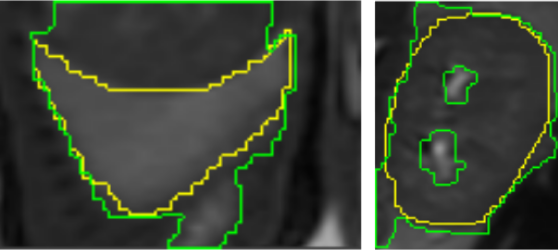
\includegraphics[scale=0.25]{pictures/grabcuts2}
    \caption{Grabcut algorithm in difficult cases. In \textit{yellow} the ground truth, in \textit{green}
    the algorithms guess \cite{BIFSeg}}
    \label{fig:minCut}
  \end{figure}
  
\end{frame}


\begin{frame}[fragile]{Graph Cuts}

  \textbf{Requires object and background pixels to have distinct intensity values}
   
  This is the case for most traditional segmentation methods
  
\end{frame}


%%%%%%%%%%%%%%%%%%%%%%%%%%%%%%%%%%%%%%%%%%%%%%%%%%%%%%%%%%%%%%%%%%%%%%%%%%%%%%%%%%%%
%%%%%%%%%%%%%%%%%%%%%%%%%%%%%%%%%%%%%%%%%%%%%%%%%%%%%%%%%%%%%%%%%%%%%%%%%%%%%%%%%%%%
%%%%%%%%%%%%%%%%%%%%%%%%%%%%%%%%%%% CNNs %%%%%%%%%%%%%%%%%%%%%%%%%%%%%%%%%%%%%%%%%%%
%%%%%%%%%%%%%%%%%%%%%%%%%%%%%%%%%%%%%%%%%%%%%%%%%%%%%%%%%%%%%%%%%%%%%%%%%%%%%%%%%%%%
%%%%%%%%%%%%%%%%%%%%%%%%%%%%%%%%%%%%%%%%%%%%%%%%%%%%%%%%%%%%%%%%%%%%%%%%%%%%%%%%%%%%

\section{Convolutional Neural Networks}

\begin{frame}[fragile]{Convolutional Neural Networks}

  \textbf{Advantages}
  \begin{itemize}
  \item Spatial operations
  \item Learning
  \item Performance
  \end{itemize}

  \textbf{Disadvantages}
  \begin{itemize}
  \item Computationally expensive
  \item Poor generalisation to unseen types
  \item Need large datasets - expensive for medical imagery
  \end{itemize}
  
\end{frame}

\begin{frame}[fragile]{Segmentation CNNs}
  
  \textbf{Classification CNNs -} gradually extract larger features from smaller ones
  \pause
  
  \textbf{U-Net CNNs -} gradually re-combine those features to produce a segmentation map

  \begin{figure}[h!]
    \centering
    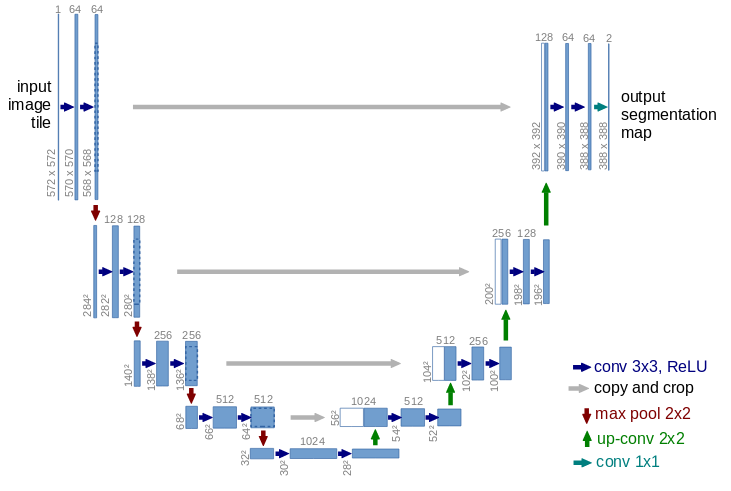
\includegraphics[scale=0.25]{pictures/U-Net}
    \caption{The U-Net architecture \cite{uNet}}
    \label{fig:minCut}
  \end{figure}

\end{frame}

\begin{frame}[fragile]{Segmentation CNNs}

  \textbf{Improvements since original U-Net}:
  \begin{itemize}
  \item Residual blocks
  \item Spatial Dropout
  \item Segmentation Layers
  \end{itemize}
  
\end{frame}

\begin{frame}[fragile]{Segmentation CNNs}

  \begin{figure}[h!]
    \centering
    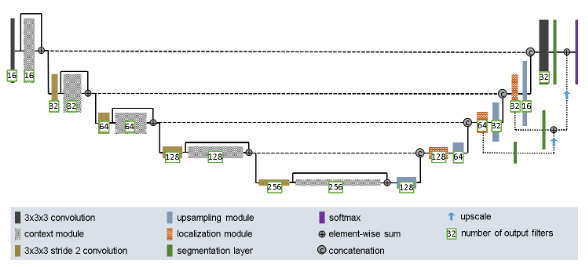
\includegraphics[scale=0.53]{pictures/isensee}
    \caption{The Isensee et al. architecture \cite{UResNet}}
    \label{fig:minCut}
  \end{figure}

  \textbf{Segmentation Layers} encourage earlier layers to produce segmentations
  
\end{frame}

%%%%%%%%%%%%%%%%%%%%%%%%%%%%%%%%%%%%%%%%%%%%%%%%%%%%%%%%%%%%%%%%%%%%%%%%%%%%%%%%%%%%
%%%%%%%%%%%%%%%%%%%%%%%%%%%%%%%%%%%%%%%%%%%%%%%%%%%%%%%%%%%%%%%%%%%%%%%%%%%%%%%%%%%%
%%%%%%%%%%%%%%%%%%%%%%%%%%%%%%% AIMS AND DESIGN %%%%%%%%%%%%%%%%%%%%%%%%%%%%%%%%%%%%
%%%%%%%%%%%%%%%%%%%%%%%%%%%%%%%%%%%%%%%%%%%%%%%%%%%%%%%%%%%%%%%%%%%%%%%%%%%%%%%%%%%%
%%%%%%%%%%%%%%%%%%%%%%%%%%%%%%%%%%%%%%%%%%%%%%%%%%%%%%%%%%%%%%%%%%%%%%%%%%%%%%%%%%%%

\section{Aims and Design}

\begin{frame}[fragile]{Aims}

  \textbf{Aims:}
  
  Minimize the disadvantages of CNNs so that they can be used for 3D image segmentation
  
  \textbf{Disadvantages}
  \begin{enumerate}
  \item Computationally expensive
  \item Poor generalisation to unseen types
  \item Need large datasets - expensive for medical imagery
  \end{enumerate}
  
\end{frame}

\begin{frame}[fragile]{BIFSeg}

  \textbf{Bounding-box Image-specific Fine-Tuning Segmentations} (BIFSeg) \cite{BIFSeg}

  Combines CNN and CRF

  Leverages user corrections
  
  \begin{enumerate}
  \item Draw bounding box around area of interest
  \item CNN and CRF give initial guess
  \item User provides correction scribbles
  \item CNN fine-tunes using corrections and gives corrected result
  \end{enumerate}
  
\end{frame}

\begin{frame}[fragile]{BIFSeg}

  \begin{figure}[h!]
    \centering
    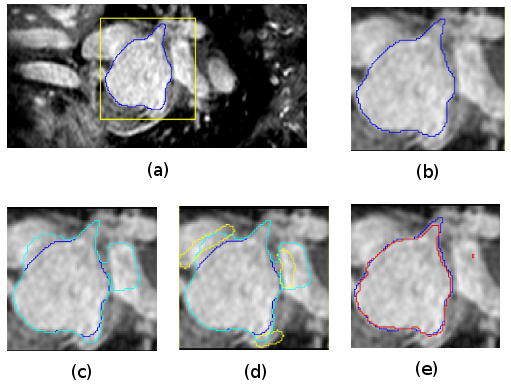
\includegraphics[scale=0.46]{pictures/heartBifSeg2}
    \caption{The steps in the BIFSeg framework. In \textit{blue} is the ground truth, in \textit{cyan} the initial guess,
      in \textit{yellow} pixels relabelled as background and in \textit{red} is the final result}
    \label{fig:minCut}
  \end{figure}
  
\end{frame}

\begin{frame}[fragile]{BIFSeg}

  \textbf{Two things going on:}
  \begin{itemize}
  \item {
    \textbf{Combining CNN and CRF}
  
    CNN softmax output used as probability values for calculating $R_{i}$
  }
    \pause
  \item{
  \textbf{Fine-Tuning CNN using CRF}
  \begin{enumerate}
  \item CNN, CRF and scribbles produce segmentation
  \item CNN trained to match segmentation
  \item Repeat steps 1 and 2 $n$ times
  \end{enumerate}
  }
  \end{itemize}
\end{frame}

\begin{frame}[fragile]{BIFSeg}


  \textbf{Fine-Tuning CNN using CRF}

  CNN loss function is \textbf{weighted} on a per-pixel basis during fine-tuning,
  such that the weight for pixel $i$ is

  \begin{equation} w_{i} = \begin{cases} 
      0 & i \in \mathbf{U} \\
      w & i \in \mathbf{S} \\
      1 & \textrm{otherwise}
   \end{cases}
  \end{equation}

  \begin{itemize}
  \item \textbf{U} - set of pixels for which the current segmentation is uncertain
  \item \textbf{S} - set of user scribbles
  \end{itemize}

  \pause
  Pixels in \textbf{U} are either \textbf{geodesically} near a scribble of opposite label
  or have $P_i$ near $0.5$
  
\end{frame}


\begin{frame}[fragile]{Design}

  \textbf{BIFSeg works on unseen object types} - though it
  needs a CNN that has learned \textbf{generalisable features}

  Performs better and with less user interaction on seen object types

  \pause
  \textbf{Unseen Types - Transfer learning}
  \begin{enumerate}
  \item Start by using a CNN trained in generalised segmentation
  \item After $n$ images have been segmented, add them to a dataset
  \item Load a new CNN with the generalised CNN weights and train it on the dataset
  \item Repeat steps 2 and 3 until all images have been segmented
  \end{enumerate}

\end{frame}

%% \begin{frame}[fragile]{Design}
  
%%   \begin{table}[h!]
%%     \centering
%%     \begin{tabular}{|l|l|}
%%       \hline
%%       \textbf{Problem}   & \textbf{Solution}         \\ \hline
%%       Computationally expensive  & Run on web server \\ 
%%       Poor generalisation  & BIFSeg \\ 
%%       Need large datasets  & Transfer Learning \\ \hline
%%     \end{tabular}
%%     \label{tab:resGen}
%%   \end{table}

%% \end{frame}

\begin{frame}[fragile]{Design}
  

  \textbf{Disadvantages}
  \begin{enumerate}
  \item Computationally expensive \onslide<2->{\checkmark (Web Server)}
  \item Poor generalisation to unseen types \onslide<3->{\checkmark (BIFSeg)}
  \item Need large datasets  \onslide<4->{\checkmark (Transfer Learning)}
  \end{enumerate}
  
\end{frame}


% Do dice loss function
% Do gridcuts
% Transfer learning


%%%%%%%%%%%%%%%%%%%%%%%%%%%%%%%%%%%%%%%%%%%%%%%%%%%%%%%%%%%%%%%%%%%%%%%%%%%%%%%%%%%%
%%%%%%%%%%%%%%%%%%%%%%%%%%%%%%%%%%%%%%%%%%%%%%%%%%%%%%%%%%%%%%%%%%%%%%%%%%%%%%%%%%%%
%%%%%%%%%%%%%%%%%%%%%%%%%%%%%%%%%%% Results %%%%%%%%%%%%%%%%%%%%%%%%%%%%%%%%%%%%%%%%
%%%%%%%%%%%%%%%%%%%%%%%%%%%%%%%%%%%%%%%%%%%%%%%%%%%%%%%%%%%%%%%%%%%%%%%%%%%%%%%%%%%%
%%%%%%%%%%%%%%%%%%%%%%%%%%%%%%%%%%%%%%%%%%%%%%%%%%%%%%%%%%%%%%%%%%%%%%%%%%%%%%%%%%%%

\section{Results}

\begin{frame}[fragile]{Seen object types}

  Evaluate performance on \textbf{seen} objects

  Train left atrium images

 
  \begin{table}[h!]
    \centering
    \begin{tabular}{|l|l|}
      \hline
      Organ   & Dice Score         \\ \hline
      Left Atrium (Initial Prediction)  & $0.872 \pm 0.025$ \\ 
      Left Atrium (With 6 scribbles)     & $0.912 \pm 0.018$ \\ 
      Liver and Spleen (Initial Prediction)  & $0.093 \pm 0.043$ \\ \hline
    \end{tabular}
    \caption{Validation scores for the generalized segmentation CNN on the organs it was trained on}
    \label{tab:resGen}
  \end{table}
  
\end{frame}



%
% Unseen object types
%

\begin{frame}[fragile]{Unseen Object Types}

  Evaluate performance on \textbf{unseen} objects

  First train a generalised segmentation CNN on:
  \begin{itemize}
  \item Left Atrium
  \item Prostate
  \item Hippocampus
  \end{itemize}
  
\end{frame}

\begin{frame}[fragile]{Unseen Object Types}

  \begin{table}[h!]
    \centering
    \begin{tabular}{|l|l|l|}
      \hline
      Organ        & Dice Score (CNN)  & Dice Score (CNN+CRF) \\ \hline
      Liver        & $0.516 \pm 0.019$ & $0.532 \pm 0.022$\\ 
      Spleen       & $0.417 \pm 0.033$ & $0.484 \pm 0.037$ \\ \hline
    \end{tabular}
    \caption{Dice scores by the generalized segmentation CNN on unseen object types with and without the CRF}
    \label{tab:resGenUnseen}
  \end{table}


  \begin{table}[h!]
    \centering
    \begin{tabular}{|l|l|l|}
      \hline
      Organ        & Dice Score (10 scribbles) & Dice Score (15 scribbles) \\ \hline
      Liver        & $0.873 \pm 0.029$ & $0.891 \pm 0.021$\\ 
      Spleen       & $0.892 \pm 0.018$ & $0.918 \pm 0.016$ \\ \hline
    \end{tabular}
    \caption{Dice scores by the generalized segmentation CNN on unseen object types, after fine-tuning with user interaction}
    \label{tab:resGenBIFUnseen}
  \end{table}
  
\end{frame}


\begin{frame}[fragile]{Unseen Object Types} 
 \begin{figure}[h!]
    \centering
    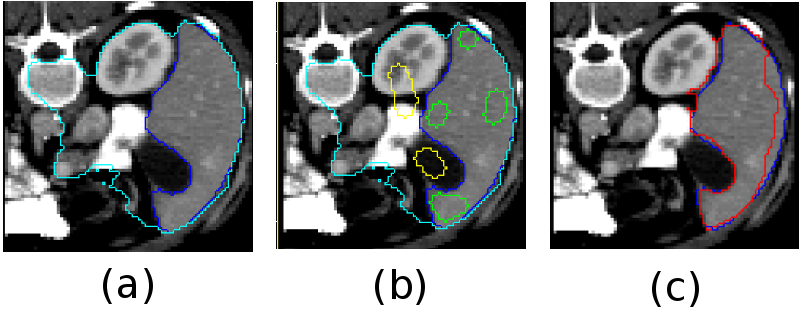
\includegraphics[scale=0.38]{pictures/genBIFSEG2}
    \caption{Segmentation of unseen object type (liver) using BIFSeg. In \textit{blue} is the ground truth,
      in \textit{yellow} are background scribbles, in \textit{green} foreground scribbles and in \textit{red} the final segmentation.
      Final Dice score over the 3D image was 0.884
    }
    \label{fig:spleenPlot}
  \end{figure}
  
\end{frame}

%
% Transfer Learning
%

\begin{frame}[fragile]{Transfer Learning}

  Evaluate performance of \textbf{transfer learning}

  Train 2 CNNs on a \textbf{small dataset} (4 training, 6 validation)
  \begin{itemize}
  \item Train one starting from scratch
  \item Train one starting from generalised CNN (transfer learning)
  \end{itemize}

\end{frame}

\begin{frame}[fragile]{Transfer Learning - Liver}
  
 \begin{figure}[h!]
    \centering
    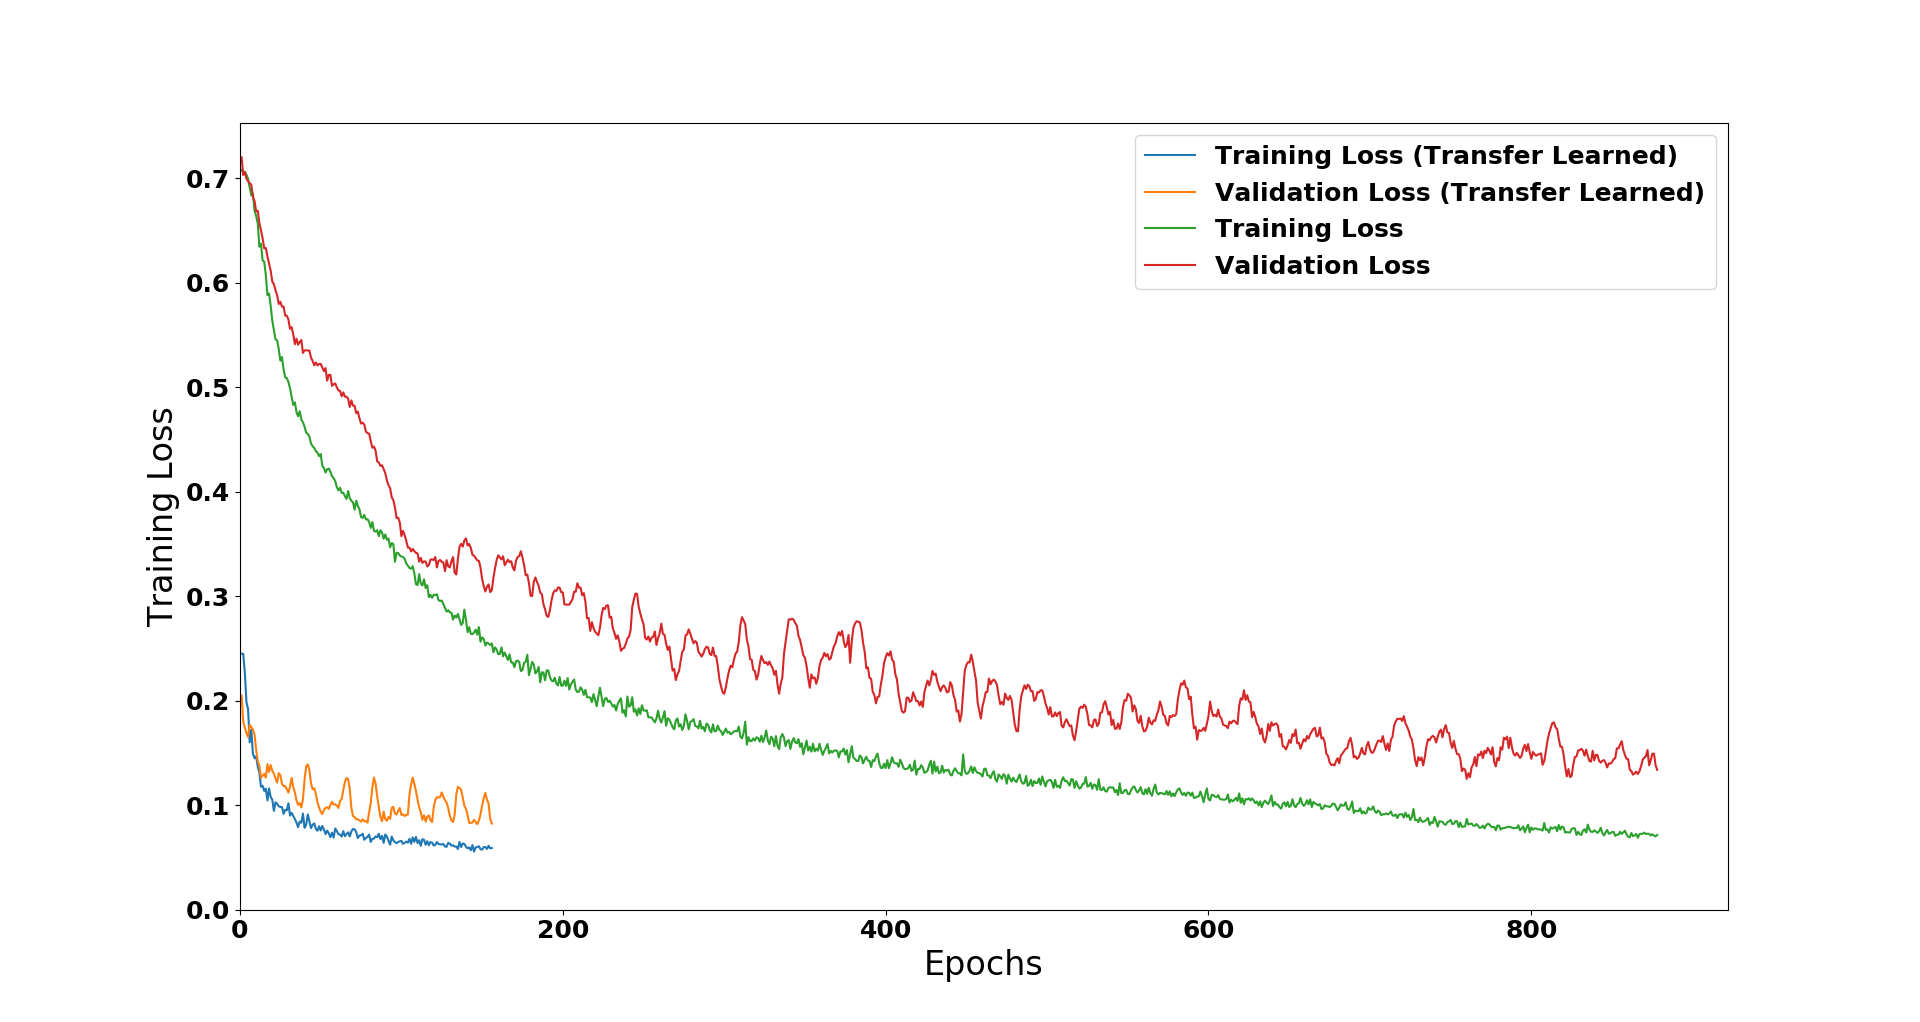
\includegraphics[scale=0.21]{pictures/transferLiver}
    \caption{Comparison of transfer learning and learning from scratch on the liver with 4 training images and 6 validation images}
    \label{fig:liverPlot}
  \end{figure}
  
\end{frame}

\begin{frame}[fragile]{Transfer Learning - Spleen}
  
 \begin{figure}[h!]
    \centering
    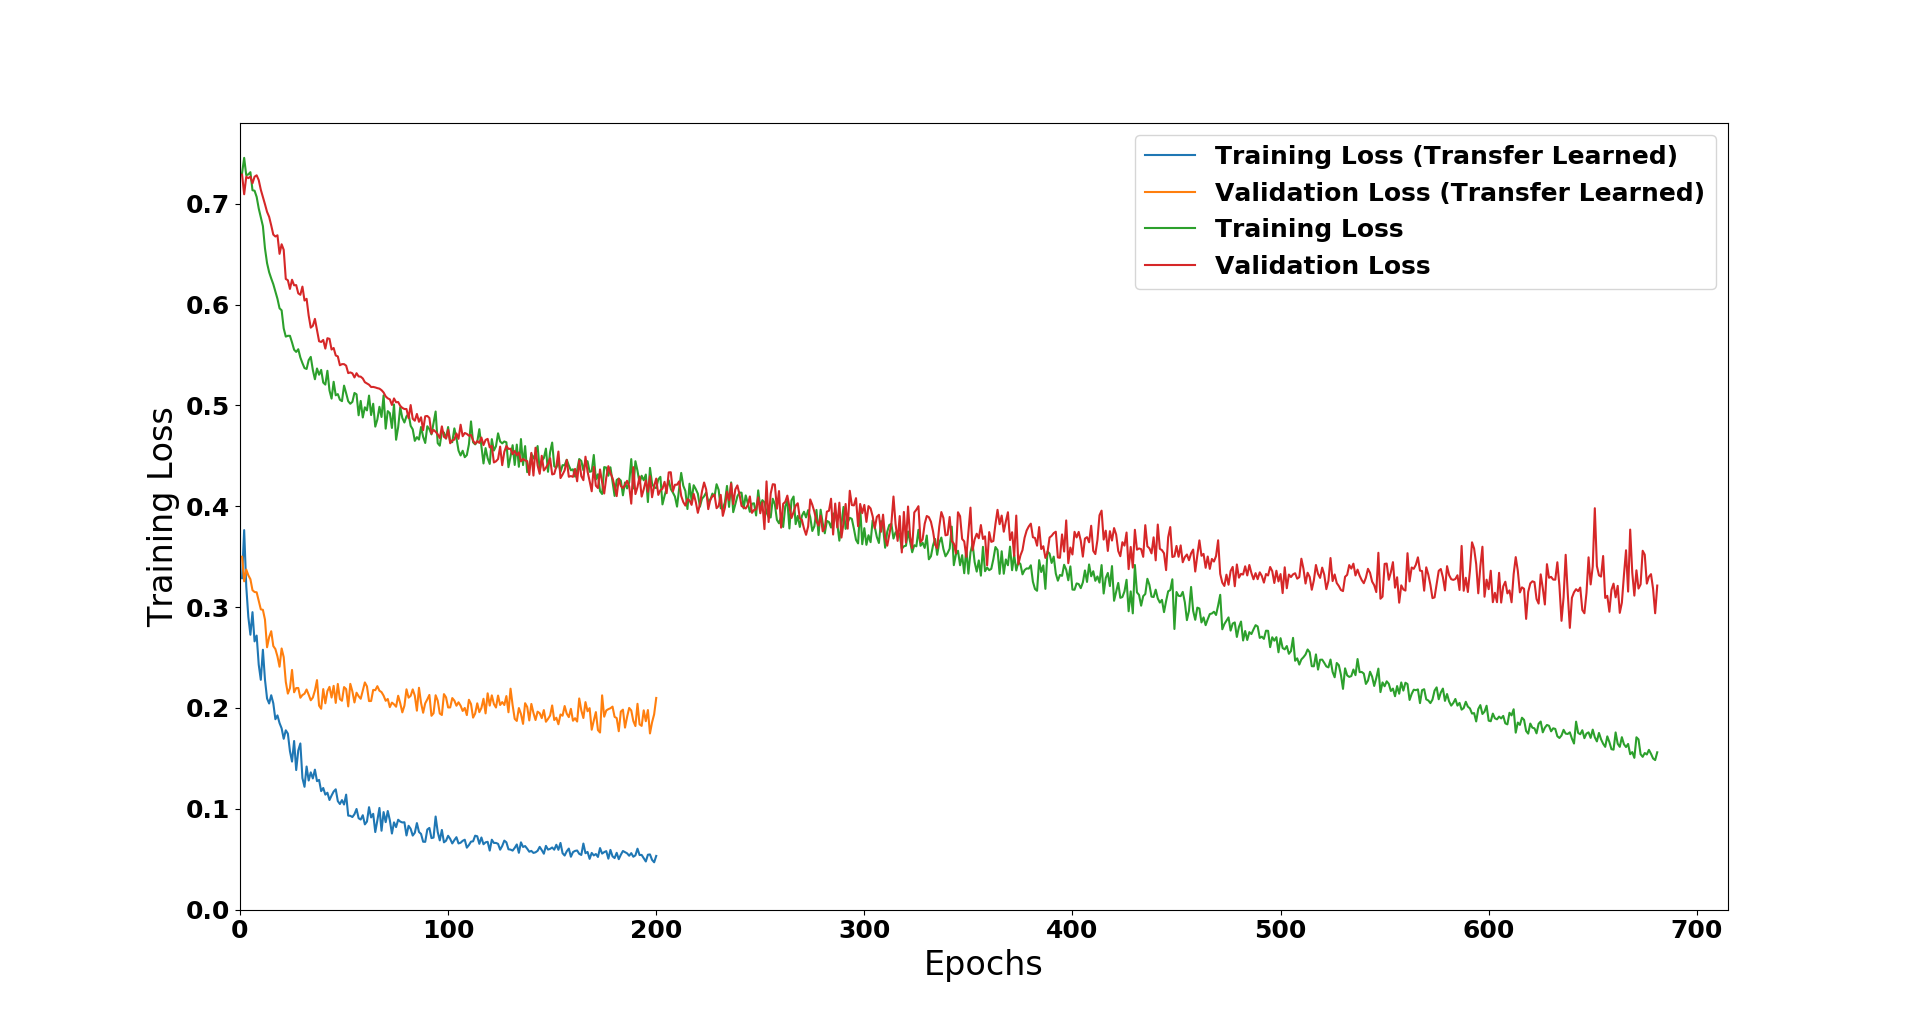
\includegraphics[scale=0.22]{pictures/transferSpleen}
    \caption{Comparison of transfer learning and learning from scratch on the spleen with 4 training images and 6 validation images}
    \label{fig:spleenPlot}
  \end{figure}
  
\end{frame}

%%%%%%%%%%%%%%%%%%%%%%%%%%%%%%%%%%%%%%%%%%%%%%%%%%%%%%%%%%%%%%%%%%%%%%%%%%%%%%%%%%%%
%%%%%%%%%%%%%%%%%%%%%%%%%%%%%%%%%%%%%%%%%%%%%%%%%%%%%%%%%%%%%%%%%%%%%%%%%%%%%%%%%%%%
%%%%%%%%%%%%%%%%%%%%%%%%%%%%%%%%% Further Work %%%%%%%%%%%%%%%%%%%%%%%%%%%%%%%%%%%%%
%%%%%%%%%%%%%%%%%%%%%%%%%%%%%%%%%%%%%%%%%%%%%%%%%%%%%%%%%%%%%%%%%%%%%%%%%%%%%%%%%%%%
%%%%%%%%%%%%%%%%%%%%%%%%%%%%%%%%%%%%%%%%%%%%%%%%%%%%%%%%%%%%%%%%%%%%%%%%%%%%%%%%%%%%

\section{Further Work}

\begin{frame}[fragile]{Further Work}
  

  \textbf{Further Work}
  \begin{itemize}
  \item Timed tests with users comparing different frameworks
  \item Temperature scaling for smoother probability distribution
  \item TLS
  \item Multiple servers with GPUs
  \end{itemize}
  
\end{frame}


%%%%%%%%%%%%%%%%%%%%%%%%%%%%%%%%%%%%%%%%%%%%%%%%%%%%%%%%%%%%%%%%%%%%%%%%%%%%%%%%%%%%
%%%%%%%%%%%%%%%%%%%%%%%%%%%%%%%%%%%%%%%%%%%%%%%%%%%%%%%%%%%%%%%%%%%%%%%%%%%%%%%%%%%%
%%%%%%%%%%%%%%%%%%%%%%%%%%%%%%%% Conclusion %%%%%%%%%%%%%%%%%%%%%%%%%%%%%%%%%%%%%%%%
%%%%%%%%%%%%%%%%%%%%%%%%%%%%%%%%%%%%%%%%%%%%%%%%%%%%%%%%%%%%%%%%%%%%%%%%%%%%%%%%%%%%
%%%%%%%%%%%%%%%%%%%%%%%%%%%%%%%%%%%%%%%%%%%%%%%%%%%%%%%%%%%%%%%%%%%%%%%%%%%%%%%%%%%%

\section{Conclusion}

\begin{frame}[fragile]{Conclusion}

  \textbf{Minimized disadvantages of CNNs}

  \textbf{Disadvantages}
  \begin{enumerate}
  \item Computationally expensive \checkmark (Web Server)
  \item Poor generalisation to unseen types \checkmark (BIFSeg)
  \item Need large datasets \checkmark (Transfer Learning)
  \end{enumerate}
  
\end{frame}

\begin{frame}[allowframebreaks]{References}

  \bibliographystyle{unsrt}
  \bibliography{sample}

\end{frame}

% REFERENCES!!!!!!!1 ESP ON IMAGES!!!!!!!!
% Maxflow needs to be more precise - breath first search? what about augmenting paths?
% Make video!!
% Make further work slides

% Extra slides:
% - Residual blocks
% - CRF - neighbouring pixels 8/26, scribble penalties

% Background
% Graph cuts
% Aims

% U-Net
% Isensee
% BIFSeg
% GridCuts


%%%%%%%%%%%%%%%%%%%%%%%%%%%%%%%%%%%%%%%%%%%%%%%%%%%%%%%%%%%%%%%%%%%%%%%%%%%%%%%%%%%%
%%%%%%%%%%%%%%%%%%%%%%%%%%%%%%%%%%%%%%%%%%%%%%%%%%%%%%%%%%%%%%%%%%%%%%%%%%%%%%%%%%%%
%%%%%%%%%%%%%%%%%%%%%%%%%%%%%%%%% Extra Slides %%%%%%%%%%%%%%%%%%%%%%%%%%%%%%%%%%%%%
%%%%%%%%%%%%%%%%%%%%%%%%%%%%%%%%%%%%%%%%%%%%%%%%%%%%%%%%%%%%%%%%%%%%%%%%%%%%%%%%%%%%
%%%%%%%%%%%%%%%%%%%%%%%%%%%%%%%%%%%%%%%%%%%%%%%%%%%%%%%%%%%%%%%%%%%%%%%%%%%%%%%%%%%%

%
% Solving CRF
%

\begin{frame}[fragile]{Conditional Random Fields}

  \textbf{How do we solve it?}

  Represent the image as a graph with
  \begin{itemize}
  \item One node per pixel
  \item One source node (object)
  \item One sink (background)
  \end{itemize}

  \pause
  and
  
  \begin{itemize}
  \item Edges between pixels have a cost $\lambda \frac{1}{r_{ij}} e^{\frac{-(X_{i}-X_{j})^2}{2\sigma^2}}$
  \item Edges between pixels and the source terminal cost  $-\log P(i \in B)$
  \item Edges between pixels and the sink terminal cost  $-\log P(i \in O)$
  \end{itemize}
  
  \textbf{A minimum cost cut} which severs the source from the sink will now minimize the cost function
  
\end{frame}

\begin{frame}[fragile]{Conditional Random Fields}
  
  \begin{figure}[h!]
    \centering
    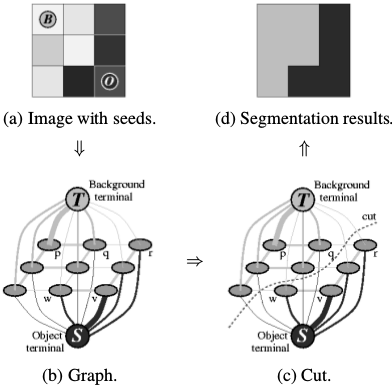
\includegraphics[scale=0.49]{pictures/graphCuts2}
    \caption{Minimum cost cut}
    \label{fig:minCut}
  \end{figure}

  
\end{frame}


\begin{frame}[fragile]{Conditional Random Fields}

  \textbf{Maxflow:} Finding the maximal flow from source to sink

  The edges that are saturated in maxflow are those in the minimal cost cut.

  \pause
  Solve with \textbf{Breadth First Search}, by gradually saturating edges
  
\end{frame}


\end{document}

\begin{frame}[fragile]{Seen Object Types}

  \begin{figure}[h!]
    \centering
    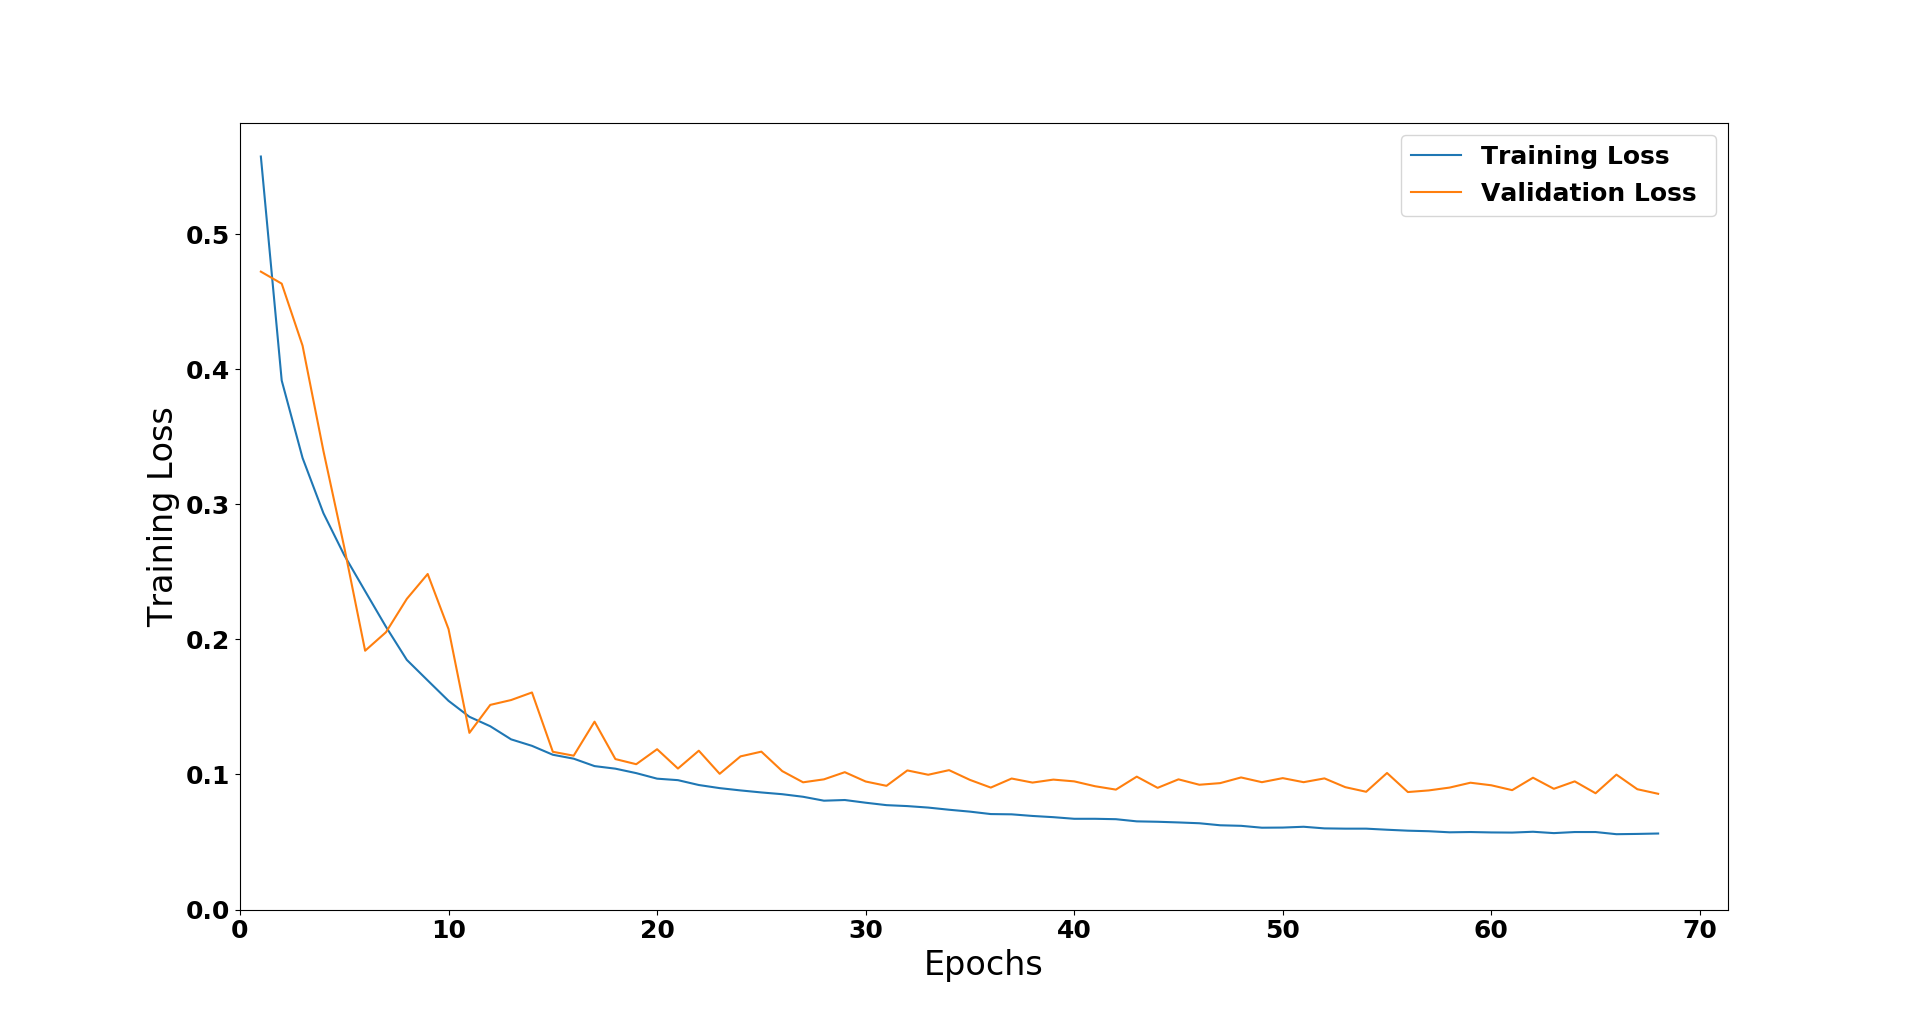
\includegraphics[scale=0.23]{pictures/heartLoss}
    \caption{Loss plot for weighted dice coefficient loss on left atrium data 
    }
    \label{fig:spleenPlot}
  \end{figure}
  
 
\end{frame}

\begin{frame}[fragile]{Unseen Object Types}

  \begin{table}[h!]
    \centering
    \begin{tabular}{|l|l|}
      \hline
      Organ        & Dice Score         \\ \hline
      Left Atrium  & $0.616 \pm 0.025$ \\ 
      Prostate     & $0.873 \pm 0.054$ \\ 
      Hippocampus  & $0.487 \pm 0.125$ \\ \hline
      All          & $0.617 \pm 0.054$ \\ \hline
    \end{tabular}
    \caption{Validation scores for the generalized segmentation CNN on the organs it was trained on}
    \label{tab:resGen}
  \end{table}
  \end{frame}
